% !TEX TS-program = pdflatex
% !TEX encoding = UTF-8 Unicode

% This is a simple template for a LaTeX document using the "article" class.
% See "book", "report", "letter" for other types of document.

\documentclass[11pt]{article} % use larger type; default would be 10pt

\usepackage[utf8]{inputenc} % set input encoding (not needed with XeLaTeX)

%%% PAGE DIMENSIONS
\usepackage{geometry} % to change the page dimensions
\geometry{a4paper} % or letterpaper (US) or a5paper or....

\usepackage{graphicx} % support the \includegraphics command and options

\usepackage{amssymb}
\usepackage{amsmath}
%%% PACKAGES
\usepackage{booktabs} % for much better looking tables
\usepackage{array} % for better arrays (eg matrices) in maths
\usepackage{paralist} % very flexible & customisable lists (eg. enumerate/itemize, etc.)
\usepackage{verbatim} % adds environment for commenting out blocks of text & for better verbatim
\usepackage{subfig} % make it possible to include more than one captioned figure/table in a single float
% These packages are all incorporated in the memoir class to one degree or another...

%%% HEADERS & FOOTERS
\usepackage{fancyhdr} % This should be set AFTER setting up the page geometry
\pagestyle{fancy} % options: empty , plain , fancy
\renewcommand{\headrulewidth}{0pt} % customise the layout...
\lhead{}\chead{}\rhead{}
\lfoot{}\cfoot{\thepage}\rfoot{}

%%% SECTION TITLE APPEARANCE
\usepackage{sectsty}
\allsectionsfont{\sffamily\mdseries\upshape} % (See the fntguide.pdf for font help)
% (This matches ConTeXt defaults)

%%% ToC (table of contents) APPEARANCE
\usepackage[nottoc,notlof,notlot]{tocbibind} % Put the bibliography in the ToC
\usepackage[titles,subfigure]{tocloft} % Alter the style of the Table of Contents
\renewcommand{\cftsecfont}{\rmfamily\mdseries\upshape}
\renewcommand{\cftsecpagefont}{\rmfamily\mdseries\upshape} % No bold!

\usepackage{amsmath}
\usepackage{graphicx}
\graphicspath{ {./pings/} }
\DeclareMathOperator*{\argmax}{arg\,max}
\DeclareMathOperator*{\argmin}{arg\,min}

\newcount\colveccount
\newcommand*\colvec[1]{
        \global\colveccount#1
        \begin{pmatrix}
        \colvecnext
}
\def\colvecnext#1{
        #1
        \global\advance\colveccount-1
        \ifnum\colveccount>0
                \\
                \expandafter\colvecnext
        \else
                \end{pmatrix}
        \fi
}

%%% END Article customizations

%%% The "real" document content comes below...

\title{Micro HW2}
\author{Michael B. Nattinger\footnote{I worked on this assignment with my study group: Alex von Hafften, Andrew Smith, Ryan Mather, and Tyler Welch. I have also discussed problem(s) with Emily Case, Sarah Bass, and Danny Edgel.}}

%\date{} % Activate to display a given date or no date (if empty),
         % otherwise the current date is printed 

\begin{document}
\maketitle

\section{Question 1}

\subsection{Prove that if the production set $Y = \{ (q,-z):f(z) \geq q \} \subset \mathbb{R}^{m+1}$ is convex, the production function $f$ is concave.}
Let $q_1 = f(z_1), q_2 = f(z_2)$. $(q_1,-z_1),(q_2,-z_2) \in Y$ by definition and by convexity $t(q_1,-z_1)+(1-t)(q_2,-z_2)\in Y,t\in(0,1)$. By definition, $f(t(z_1)+(1-t)(z_2)) \geq tq_1 + (1-t) q_2 = tf(z_1) + (1-t)f(z_2)$ so f is concave.

\subsection{Prove that if $f$ is concave, the cost function is convex in $q$.}
We can fix $w \in \mathbb{R}^k$ Let $q_1,q_2 \in \mathbb{R}$ Let $z_1,z_2$ be $\argmin\limits_{z:f(x)\geq q_1} w \cdot z, \argmin\limits_{z:f(x)\geq q_2} w \cdot z.$

By the concavity of $f$, for $t \in (0,1)$ we have $f(tz_1 + (1-t)z_2) \geq tf(z_1) + (1-t)f(z_2) \geq tq_1 + (1-t)q_2.$  Therefore $ t c(q_1,w) + (1-t)c(q_2,w) \leq c(tq_1+ (1-t) q_2,w)$ because we can produce at least $tq_1 + (1-t)q_2$ goods by using $(t(z_1) + (1-t)(z_2))$ inputs.

\section{Question 2}
\subsection{Draw Y}
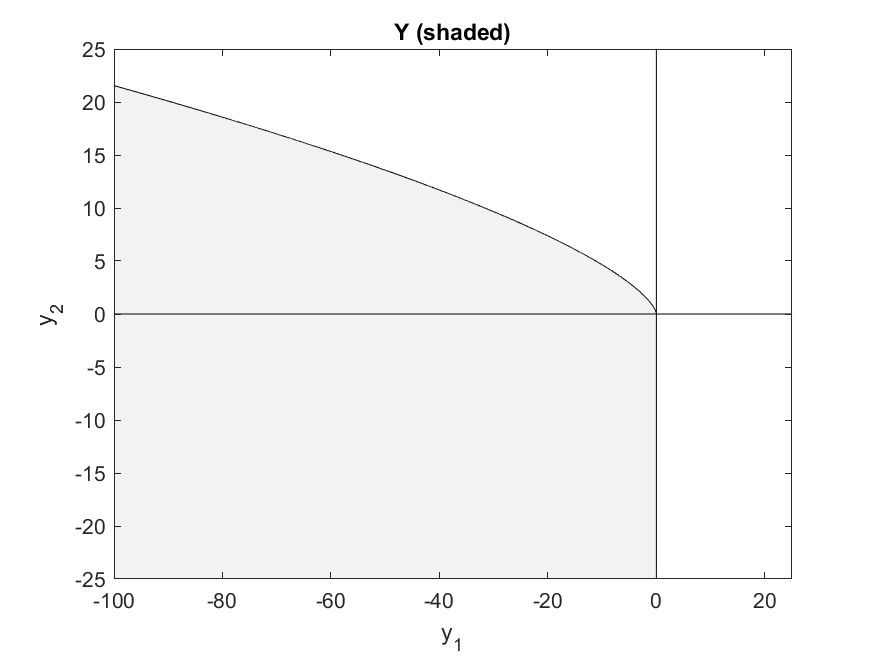
\includegraphics{Y}
The shaded area in the above figure is $Y$ graphed in Matlab, for a sample value of $B=1$.

\subsection{Solve the firm's profit maximization problem to find $\pi (p)$ and $Y^{*}(p).$}
The firm chooses production to maximize profit: $\max\limits_{-y_1,y_2 \in \mathbb{R}_{+}} p \cdot (y_1,y_2)^{'}$ s.t. $y_2 \leq B(-y_1)^{2/3}$. Since profits are strictly increasing in $y_2$ the profit maximizing firm will set $y_2 =  B(-y_1)^{2/3}$. We will also write $-y_1 = z$. Our optimization problem thus becomes: $\max\limits_{q\in\mathbb{R}_{+}} p \cdot (-q, Bq^{2/3})^{'}.$ Taking the firm's first order conditions, we find that $0 = \frac{d \pi(q)}{dq} = 0 \Rightarrow \frac{d }{dq}\left(  -p_1 q + p_2 Bq^{2/3}\right)  = 0 \Rightarrow -p_1 + (2/3)p_2 B q^{-1/3} = 0 \Rightarrow q = \left(\frac{Bp_2}{ (3/2) p_1} \right)^{3}.$ This production yields the maximum profits given $p$, which we can compute as:\\ $\pi(p) = p_1\left(\frac{Bp_2}{ (3/2) p_1} \right)^{3} + p_2 B\left(\frac{Bp_2}{ (3/2) p_1} \right)^{2},$ since $Y^{*}(p) = \left(\left(\frac{Bp_2}{ (3/2) p_1} \right)^{3},B\left(\frac{Bp_2}{ (3/2) p_1} \right)^{2}\right)^{'}$.

\subsection{Verify that $\pi(p)$ is homogeneous of degree 1, and $y(p)$ is homogeneous of degree 0.}
$\pi(\lambda p) = \lambda p_1\left(\frac{B\lambda p_2}{ (3/2) \lambda p_1} \right)^{3} + \lambda p_2 B\left(\frac{B\lambda p_2}{ (3/2) \lambda p_1} \right)^{2} = \lambda (p_1\left(\frac{Bp_2}{ (3/2) p_1} \right)^{3} + p_2 B\left(\frac{Bp_2}{ (3/2) p_1} \right)^{2}) = \lambda \pi(p)$ so $\pi(p)$ is homogeneous of degree 1. \\
$y(\lambda p) = \left(\left(\frac{B \lambda p_2}{ (3/2) \lambda p_1} \right)^{3},B\left(\frac{B\lambda p_2}{ (3/2) \lambda p_1} \right)^{2}\right)^{'} = \left(\left(\frac{Bp_2}{ (3/2) p_1} \right)^{3},B\left(\frac{Bp_2}{ (3/2) p_1} \right)^{2}\right)^{'} = y(p) $ so $y(p)$ is homogeneous of degree 0.

\subsection{Verify that $y_1(p) = \frac{\partial \pi}{\partial p_1}$ and $y_2(p) = \frac{\partial \pi}{\partial p_2}$.}
\begin{align*}
\frac{\partial \pi}{\partial p_1} &= \frac{\partial }{\partial p_1}\left( p_1\left(\frac{Bp_2}{ (3/2) p_1} \right)^{3} + p_2 B\left(\frac{Bp_2}{ (3/2) p_1} \right)^{2}\right) \\
&= \left(\frac{Bp_2}{ (3/2) p_1} \right)^{3} - 3p_1\left(\frac{Bp_2}{ (3/2) p_1} \right)^{2} \left(\frac{Bp_2}{ (3/2)p_{1}^2}\right) - 2p_2 B\left(\frac{Bp_2}{ (3/2) p_1} \right)\left(\frac{Bp_2}{ (3/2) p_{1}^2}\right)
\end{align*}

\section{Question 3}

\end{document}
